\section{Setup}
\label{sec:Setup}
In the following the two setups used are briefly explained. 

\subsection{UV/VIS setup}

In the following the UV/VIS setup is briefly explained. As the used setup was fully automated and performed the calculations on 
itself, the mathematical operations are not covered in the following section.

\begin{figure}[ht]
    \centering
    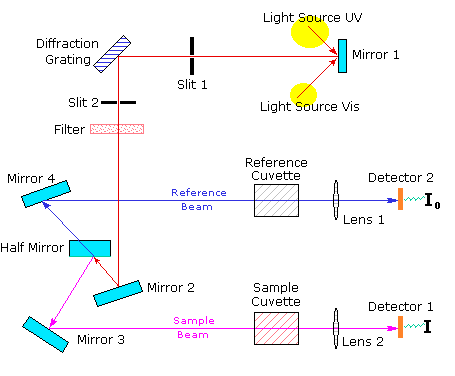
\includegraphics[width = 13cm]{Bilder/Grundlagen/UVVISsetup.png}
    \caption{Schematic representation of a UV/VIS absorption spectroscopy setup}
    \label{fig:setupUVVIS}
\end{figure}

The setup contains of several components as shown in \cref{fig:setupUVVIS}. The setup will be explained following the path of light.
The light source generates the light which is split in to two beams. One beam is guided onto a cuvette with solvent and the observed material.
The second beam is guided onto a cuvette with solvent as a reference. Afterwards, from the two spectra
-- produced by scanning and selecting wavelength with a diffracting grating-- the absorbance is calculated. 

\subsection{Transient absorption spectroscopy setup}

In the following, the setup used for transient absorption is characterized. 

The pump pulse exiting the sample as described in \cref{sec:TheoTransAbs}, is generated by a pulsed laser with a wavelength of \SI{520}{\nano\meter} as depicted in \cref{fig:TRANSsetup}.
Afterwards, two mirrors guide the beam onto the sample and afterwards the puls is absorbed by the iris. The probe puls generated in a \SI{450}{\nano\meter} is  also guided by two different mirrors onto the sample. 
The detector detects the intensity of the beam after passing the sample. The time of the pulses is controlled by a computer. 

The computer orders to generate a train of pulses, alternating a probe pulse with and without a pump pulse before as depicted in \cref{fig:PulseTrain}. This leads to having a reference with and without pump pulse before. The difference of the two is the effect investigated by transient absorption spectroscopy. 
The temporal distance between the two pulses is varied with the computer.
\begin{figure}[ht]
    \centering
    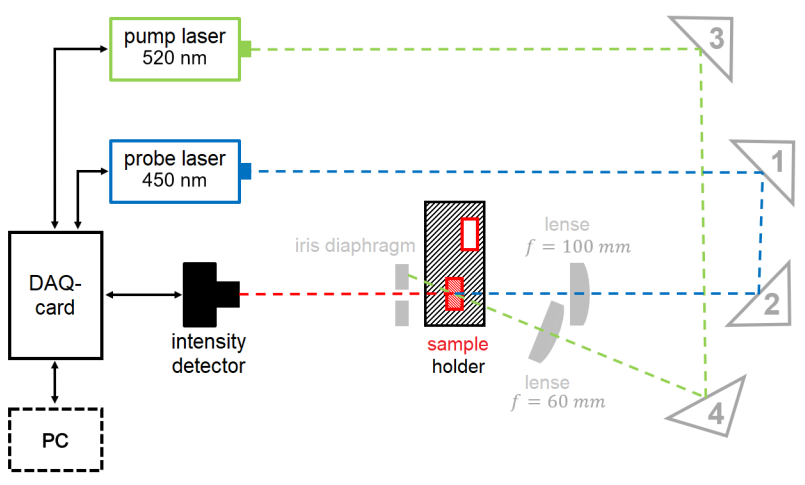
\includegraphics[width = 13cm]{Bilder/Grundlagen/TRANSsetup.png}
    \caption{Schematic representation of the transient absorption spectroscopy setup}
    \label{fig:TRANSsetup}
\end{figure}

\begin{figure}[h]
    \centering
    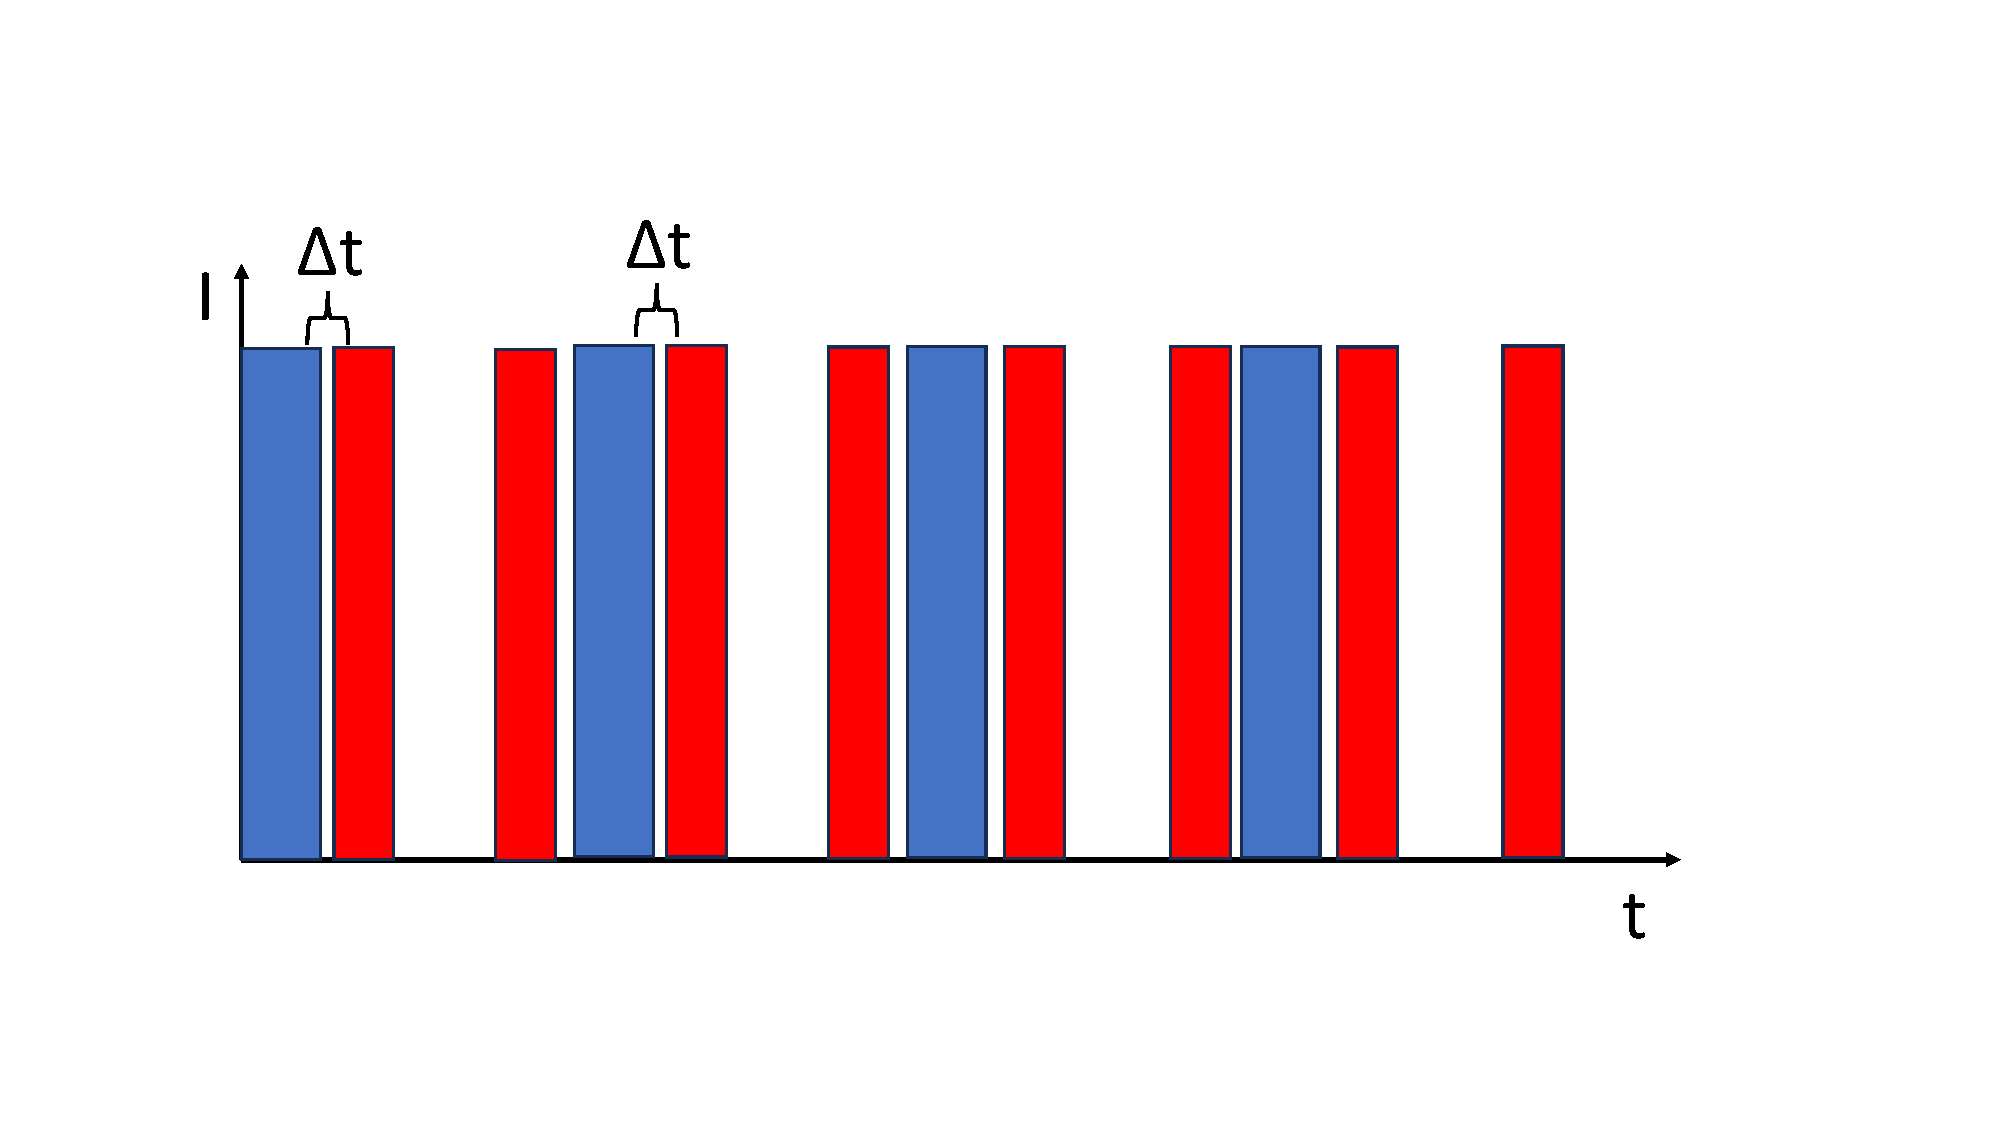
\includegraphics[width = 13cm]{Bilder/Grundlagen/PulseTrain.pdf}    
    \caption{Schematic representation of a train of probe and pump pulse. The probe pulses (red) are shifted in time compared to the pump pulses (blue).}
    \label{fig:PulseTrain}
\end{figure}

